\section{Spracherweiterungen}

Kurze Beschreibung der Erweiterungen der Sprache. Grundsatz: Kompatibilität beibehalten!

\subsection{Pre-/Postconditions}
Funktionen/Prozeduren mit Pre und Postconditions versehen können.


\begin{lstlisting}[caption=Definieren von pre-/postconditions]
proc divide(in copy m:int32, in copy n:int32, out ref q:int, out ref r:int32)
requires [n > 0, call unnecessary(m, n)]
ensures [r >= 0]
{
    q init := 0;
    r init := m;

    while(r >= n) {
        q := q+1;
        r := r-n;
    }
}
\end{lstlisting}



\subsection{Pure Operationen}
Funktionen/Prozeduren als pur kenzeichnen. -- keine Veränderung von State erlaubt. Dürfen in conditions verwendet werden
\begin{lstlisting}[caption=Pure Operationen]
pure fun unnecessary(in copy a:int32, in copy b:int32)
returns var v:bool 
{
    v init := true
}
\end{lstlisting}


%\newpage

%\begin{figure*}[h]
%	\begin{center}
%		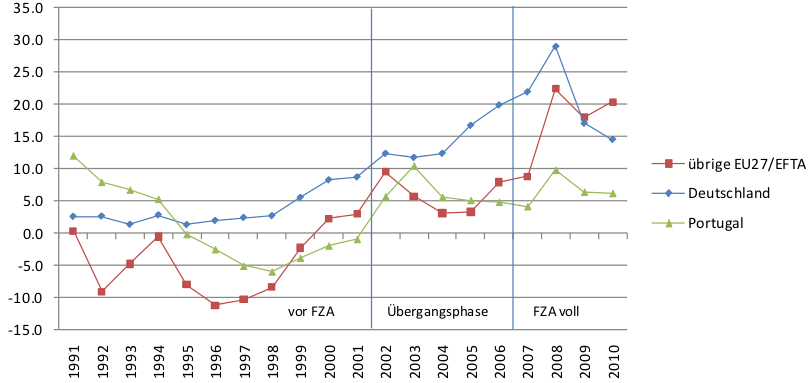
\includegraphics[width=0.9\textwidth]{images/Zuwanderungssaldo_Bericht_2.png}
%	\end{center}
%	\caption{Verlauf der Zuwanderung nach Herkunftsländern in Tausend \cite[S. 18]{ADMIN:Bericht}}
%	\label{fig:zuwanderungsaldi}
%\end{figure*}

